%% This is file `DEMO-TUDaThesis.tex' version 2.09 (2020/03/13),
%% it is part of
%% TUDa-CI -- Corporate Design for TU Darmstadt
%% ----------------------------------------------------------------------------
%%
%%  Copyright (C) 2018--2020 by Marei Peischl <marei@peitex.de>
%%
%% ============================================================================
%% This work may be distributed and/or modified under the
%% conditions of the LaTeX Project Public License, either version 1.3c
%% of this license or (at your option) any later version.
%% The latest version of this license is in
%% http://www.latex-project.org/lppl.txt
%% and version 1.3c or later is part of all distributions of LaTeX
%% version 2008/05/04 or later.
%%
%% This work has the LPPL maintenance status `maintained'.
%%
%% The Current Maintainers of this work are
%%   Marei Peischl <tuda-ci@peitex.de>
%%   Markus Lazanowski <latex@ce.tu-darmstadt.de>
%%
%% The development respository can be found at
%% https://github.com/tudace/tuda_latex_templates
%% Please use the issue tracker for feedback!
%%
%% ============================================================================
%%
% !TeX program = lualatex
%%

\documentclass[
	english,
	ruledheaders=section,%Ebene bis zu der die Überschriften mit Linien abgetrennt werden, vgl. DEMO-TUDaPub
	class=report,% Basisdokumentenklasse. Wählt die Korrespondierende KOMA-Script Klasse
	thesis={type=bachelor},% Dokumententyp Thesis, für Dissertationen siehe die Demo-Datei DEMO-TUDaPhd
	accentcolor=1b,% Auswahl der Akzentfarbe
	custommargins=true,% Ränder werden mithilfe von typearea automatisch berechnet
	marginpar=false,% Kopfzeile und Fußzeile erstrecken sich nicht über die Randnotizspalte
	%BCOR=1mm,%Bindekorrektur, falls notwendig
	parskip=half-,%Absatzkennzeichnung durch Abstand vgl. KOMA-Sript
	fontsize=11pt,%Basisschriftgröße laut Corporate Design ist mit 9pt häufig zu klein
	DIV=14,
%	logofile=example-image, %Falls die Logo Dateien nicht vorliegen
]{tudapub}
\usepackage{datetime2}


% Der folgende Block ist nur bei pdfTeX auf Versionen vor April 2018 notwendig
%\usepackage{iftex}
%\ifPDFTeX
%	\usepackage[utf8]{inputenc}%kompatibilität mit TeX Versionen vor April 2018
%\fi

%%%%%%%%%%%%%%%%%%%
%Sprachanpassung & Verbesserte Trennregeln
%%%%%%%%%%%%%%%%%%%
\usepackage[english, main=ngerman]{babel}
\usepackage[autostyle]{csquotes}% Anführungszeichen vereinfacht
\usepackage{microtype}
\usepackage[super]{nth} % converts Dec \nth{1} to Dec 1st (with st as superscript)


%%%%%%%%%%%%%%%%%%%
%Literaturverzeichnis
%%%%%%%%%%%%%%%%%%%
\usepackage[style=authoryear-ibid,backend=biber]{biblatex}   % Literaturverzeichnis
\DeclareLanguageMapping{english}{english-apa}
\bibliography{references}
\AtBeginBibliography{\setcounter{maxnames}{10}} % Im Literaturverzeichnis nenne mehr als 2 Autoren
\counterwithout{footnote}{chapter} % Zähle Fußnoten über gesamtes Dokument hoch


%%%%%%%%%%%%%%%%%%%
%Paketvorschläge Tabellen
%%%%%%%%%%%%%%%%%%%
%\usepackage{array}     % Basispaket für Tabellenkonfiguration, wird von den folgenden automatisch geladen
\usepackage{tabularx}   % Tabellen, die sich automatisch der Breite anpassen
\usepackage{longtable} % Mehrseitige Tabellen
\usepackage{xtab,afterpage}
%\usepackage{xltabular} % Mehrseitige Tabellen mit anpassarer Breite
\usepackage{booktabs}   % Verbesserte Möglichkeiten für Tabellenlayout über horizontale Linien
\usepackage{tikz}       % Graphen zeichnen
\usepackage{enumitem, hyperref}   % for referencing in enumerate und description
\usepackage{amsmath}    % https://tex.stackexchange.com/questions/32140/how-to-write-a-function-piecewise-with-bracket-outside
% https://texblog.org/2012/03/21/cross-referencing-list-items/
\usepackage[acronym,shortcuts,nonumberlist,nomain]{glossaries} % for Abbreviations (Acronyms)

%%%%%%%%%%%%%%%%%%%
%Paketvorschläge Mathematik
%%%%%%%%%%%%%%%%%%%
%\usepackage{mathtools} % erweiterte Fassung von amsmath
%\usepackage{amssymb}   % erweiterter Zeichensatz
%\usepackage{siunitx}   % Einheiten

% Customs
%\usepackage[singlespacing]{setspace}
\usepackage[]{setspace}
%\usepackage[printonlyused]{acronym}

%Formatierungen für Beispiele in diesem Dokument. Im Allgemeinen nicht notwendig!
\let\file\texttt
\let\code\texttt
\let\tbs\textbackslash

\usepackage{pifont}% Zapf-Dingbats Symbole
\newcommand*{\FeatureTrue}{\ding{52}}
\newcommand*{\FeatureFalse}{\ding{56}}

\makeglossaries

\begin{document}

\Metadata{
	title=Automatic evaluation of Enterprise-GenAI Applications success,
	author=Marcel Pfeiffer
}

\pagenumbering{gobble}

\title{Automatic evaluation of Enterprise-GenAI Applications success}

\studentID{2912332}
\author[M. Pfeiffer]{Marcel Pfeiffer}%optionales Argument ist die Signatur,
\birthplace{Koblenz}%Geburtsort, bei Dissertationen zwingend notwendig
\reviewer{Prof. Dr. Peter Buxmann \and Prof. Dr. X Y}%Gutachter

%Diese Felder erden untereinander auf der Titelseite platziert.
%\department ist eine notwendige Angabe, siehe auch dem Abschnitt `Abweichung von den Vorgaben für die Titelseite'
\department{wi} % Das Kürzel wird automatisch ersetzt und als Studienfach gewählt, siehe Liste der Kürzel im Dokument.
\institute{Wirtschatsinformatik}
\group{Software \& Digital Business}

\submissiondate{\today}
\examdate{\today}

%	\tuprints{urn=1234,printid=12345}
%	\dedication{Für alle, die \TeX{} nutzen.}

\maketitle

\affidavit


%---------------------------------------------------------------------%
%----------------------------- Abstract ------------------------------%
%---------------------------------------------------------------------%
\chapter*{Abstract}
Der Abstract fasst den Inhalt der Abschlussarbeit auf maximal einer halben Seite zusammen. Ziel des Abstracts ist es, dem Leser einen möglichst schnellen Überblick über den Inhalt der Arbeit zu verschaffen und die wesentlichen Ergebnisse darzustellen. Mögliche Inhalte sind die Zielsetzung oder Forschungsfrage der Arbeit, verwendete Theorien, die verwendete Methodik sowie eine kurze Darstellung der zentralen Ergebnisse und Beiträge.

\tableofcontents


\pagenumbering{Roman}

%---------------------------------------------------------------------%
%-------------------------- List of Figures --------------------------%
%---------------------------------------------------------------------%

\listoffigures
\addcontentsline{toc}{chapter}{Abbildungsverzeichnis}           %Kapitel bekommt keine Nummerierung und wird trotzdem
                                                                %ins Inhaltsverzeichnis aufgenommen
%---------------------------------------------------------------------%
%--------------------------- List of Tables --------------------------%
%---------------------------------------------------------------------%

\listoftables
\addcontentsline{toc}{chapter}{Tabellenverzeichnis}           %Kapitel bekommt keine Nummerierung und wird trotzdem
                                                                %ins Inhaltsverzeichnis aufgenommen

%---------------------------------------------------------------------%
%----------------------- List of Abbreviations -----------------------%
%---------------------------------------------------------------------%
\chapter*{Abkürzungsverzeichnis}
\addcontentsline{toc}{chapter}{Abkürzungsverzeichnis}           %Kapitel bekommt keine Nummerierung und wird trotzdem
                                                                %ins Inhaltsverzeichnis aufgenommen

\begin{xtabular}{ll}
IS					&	Information Systems\\
TUD					&	Technische Universität Darmstadt\\
KMS                 &   Knowledge Management System \\

\end{xtabular} 

%---------------------------------------------------------------------%
%---------------------------- Introduction ---------------------------%
%---------------------------------------------------------------------%

\onehalfspacing
\chapter{Einleitung}
% Umstellen auf arabische Seitenzahlen. Die Anzahl der bisherigen
% Seiten wird zwischengespeichert, da die römische Nummerierung am
% Ende des Dokuments fortgesetzt werden soll.
\newcounter{seitenzahlroemisch}
\setcounter{seitenzahlroemisch}{\value{page}}
\pagenumbering{arabic}

Die Datei \file{DEMO-TUDaThesis.tex} ist ein Template für Abschlussarbeiten im Stil des Corporate Designs der TU Darmstadt.
Sie ist Teil des TUDa-CI-Bundles wurde vom in Teilen tuddesign-Paket von C.~v.~Loewenich und J.~Werner inspiriert.

 \section{Abbildungen}
Abbildungen sollten generell linksbündig in das Dokument eingefügt werden. Die Abbildungs-beschriftung steht dabei unter der Abbildung und ist ebenfalls linksbündig auszurichten. Eine Beschriftung der Abbildungen mit der Abkürzung "Abb." ist ebenfalls möglich. Abbildungen (bzw. ihre Beschriftungen) werden von einer Leerzeile gefolgt, um den Abstand zum nachfolgenden Text zu wahren.

Beispiele:

 
\begin{figure}[ht]
     \centering
     
\includegraphics[]{images/Picture 1.png}
     \caption{Logo des Fachgebiets Wirtschaftsinformatik}
     \label{fig:logo}
\end{figure}

\begin{figure}[ht]
     \centering
     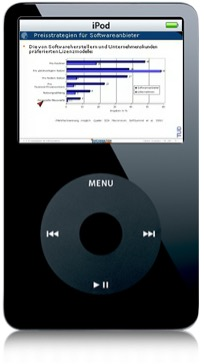
\includegraphics[]{images/Picture 1.jpg}
     \caption{Video-Podcast der Vorlesung Internet Economics auf einem iPod}
     \label{fig:logo2}
\end{figure}

\section{Zitierungen}
Wörtliche Zitate, die sich über mind. drei Textzeilen erstrecken, sind mit der "Zitat" zu formatieren. Alle anderen Zitate erhalten die gleiche Formatierung wie der restliche Fließtext \parencite{buxmann2015softwareindustrie}.

%---------------------------------------------------------------------%
%------------------------------ Theoretical Background ---------------%
%---------------------------------------------------------------------%
\chapter{Theoretical Background}
In order to gain a deeper understanding of what determines the success of an enterprise Gen-AI system, we will first look at the success of IS in general. Afterwards, we will dive deeper into the context of KMS and specifically enterprise GenAI systems and apply the more general theories to them. This will help us define and categorize the software features we are going to implement out during our artifact development.
\section{Technology acceptance and IS success}
To better understand the success of IS we will have a look at two models. The IS success model \parencite{DeloneMcLean2003ISSuccessTenYearUpdate} focuses on the success of an IS in an organizational context, whereas the technology acceptance model (TAM) deals with the question, which determinants lead to the acceptance and use of an IS by a single user.
\begin{figure}[h!]
    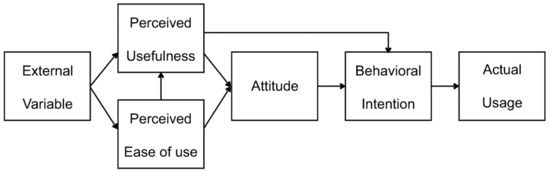
\includegraphics[width=1\linewidth]{images/TAM.png}
    \caption{Technology acceptance model}
    \label{fig:enter-label}
\end{figure}
\\
Looking at the TAM there are two determinants that influence the use of an IS - the \textit{perceived usefulness} (PU) and the \textit{perceived ease of use} (PEU). The PU describes the degree to which a person believes that using a particular system would provide some use for her or him \parencite{Davis1989MISQ}. In an enterprise context this usually means the conviction that the use of the IS has a beneficial influence on the own job performance. The second determinant, the \textit{perceived ease of use} (PEU), refers to "the degree to which a person believes that using a particular system would be free of effort" \parencite[p.~320]{Davis1989MISQ}. This idea relates to the user's assessment of the mental effort required to learn and operate the system. If a system is intuitive, straightforward and does not require extensive training to use, it will be perceived as easy to use.\\ A crucial aspect of the TAM is the relationship between these two determinants. Davis argues that the PEU has a direct, positive influence on the PU. A system that is easier to use is also perceived as more useful, partly because the user can invest less effort in the mechanics of using the system and more in the actual task at hand. Both PU and PEU then influence the user's \textit{attitude toward using} the system, which in turn shapes the \textit{behavioral intention to use} and ultimately leads to the \textit{actual system use}.However, it is important to note that a consistent finding in TAM research is that PU has a significantly stronger influence on usage intention and actual use than PEU \parencite{Davis1989MISQ}. While ease of use is important, the ultimate driver for acceptance is the user's belief that the system will help them perform their job better.\\
\\
Now that we know which factors lead to the use of an IS by a single person, we will shift our perspective to the factors that determine its use and overall success within an organizational context.
Following DeLone and McLean \parencite{DeloneMcLean2003ISSuccessTenYearUpdate} there are 6 interrelated factors that determine the success of an IS in an organizational context: \textit{system quality, information quality, service quality, intention to use and actual system use, user satisfaction and the net benefits} of the IS.\\
\begin{figure}[h!]
    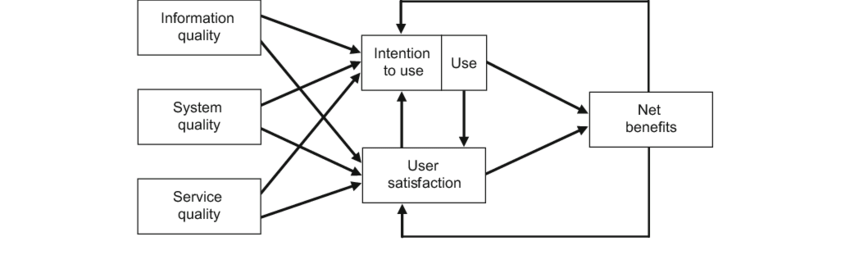
\includegraphics[width=1\linewidth]{images/ISSuccess.png}
    \caption{IS Success Model}
    \label{fig:enter-label}
\end{figure}
\\
\textit{System quality} means the quality of the IS in terms of technical performance. Typical measures for system quality would be, for example, response time, reliability, ease of use, or hardware utilization.\\
\textit{Information quality} refers to the quality of the information provided by the IS. This includes, for example, the usefulness, timeliness, precision, completeness, and relevance of the information provided by the system.\\
\textit{Service quality} means the quality of the support that users receive from the IS department or service provider. It became an important success dimension with the rise of end-user computing, where the IS function provides services in addition to products. This dimension is often measured by the support staff's responsiveness, assurance, and empathy.
\\
These three aspects of the quality of an information system directly influence the \textit{intention to use} and the actual \textit{system use} as well as the \textit{user satisfaction}. Here, it is important to differentiate between the two concepts of use. \textit{Intention to use} is an attitudinal measure, representing a user's plan or predisposition to engage with a system. In contrast, \textit{system use} is a behavioral measure of the actual interaction, capturing metrics like frequency, duration, or the breadth of features used. This distinction is particularly crucial in an enterprise context. For a system where use is voluntary, a user's intention is a strong predictor of their actual use. However, if a system's use is mandatory, simply measuring that it is being used is not very insightful. In that scenario, assessing the nature of the use (e.g., are users leveraging advanced features?) or their underlying intention to use the system properly becomes a more telling indicator of true acceptance 
\parencite{DeloneMcLean2003ISSuccessTenYearUpdate}. Both use and intention are linked with \textit{user satisfaction}. A positive experience during system use leads to higher satisfaction, which in turn reinforces the intention for continued and more extensive use in the future. In an organizational context, this user satisfaction is heavily influenced by the system's perceived impact on job performance, such as an increase in productivity. Therefore, the combination of active system use and high user satisfaction is what generates \textit{net benefits}.\\
This process, however, is not a one-way street. The model includes a crucial feedback loop: the \textit{net benefits} that users perceive will in turn influence their future \textit{user satisfaction} and \textit{intention to use}. When users see that a system is delivering real value, it reinforces their positive attitude towards the system. This creates a virtuous cycle, where a successful system's value is constantly reinforced and grown over time.
\newpage
\section{Knowledge Management Systems acceptance success}
Now that we have a solid understanding of IS acceptance and success in general we are going to have a closer look at knowledge management systems (KMS) in particular enterprise GenAI systems. We'll start of with some definitions that will help us understand what KM and KMS are. "Knowledge is an evolving mix of framed experience, values, contextual information, and expert insight that provides a framework for evaluating and incorporating new experiences and information". This means that knowledge is a key key factor in the devision-making processes e.g. in enterprises. Knowledge Management on the other hand "is the practice of selectively applying knowledge from previous experiences of decision making to current and future decision making activities with the express purpose of improving the organization’s effectiveness". KMS in the end can be defined as "IT-based systems developed to support and enhance the organizational processes of knowledge creation, storage/retrieval, transfer and application". Overall we can conclude that KMS are systems that support the decision making process e.g. in a company by managing and selectively providing knowledge to their users. Since KMS are by definition a specialized form of IS we can simply apply the ISSM to them.\\
Following Jennex and Olfman we can extend the three quality factors to gain a better understanding
of knowledge management success.\\
\begin{figure}
    \centering
    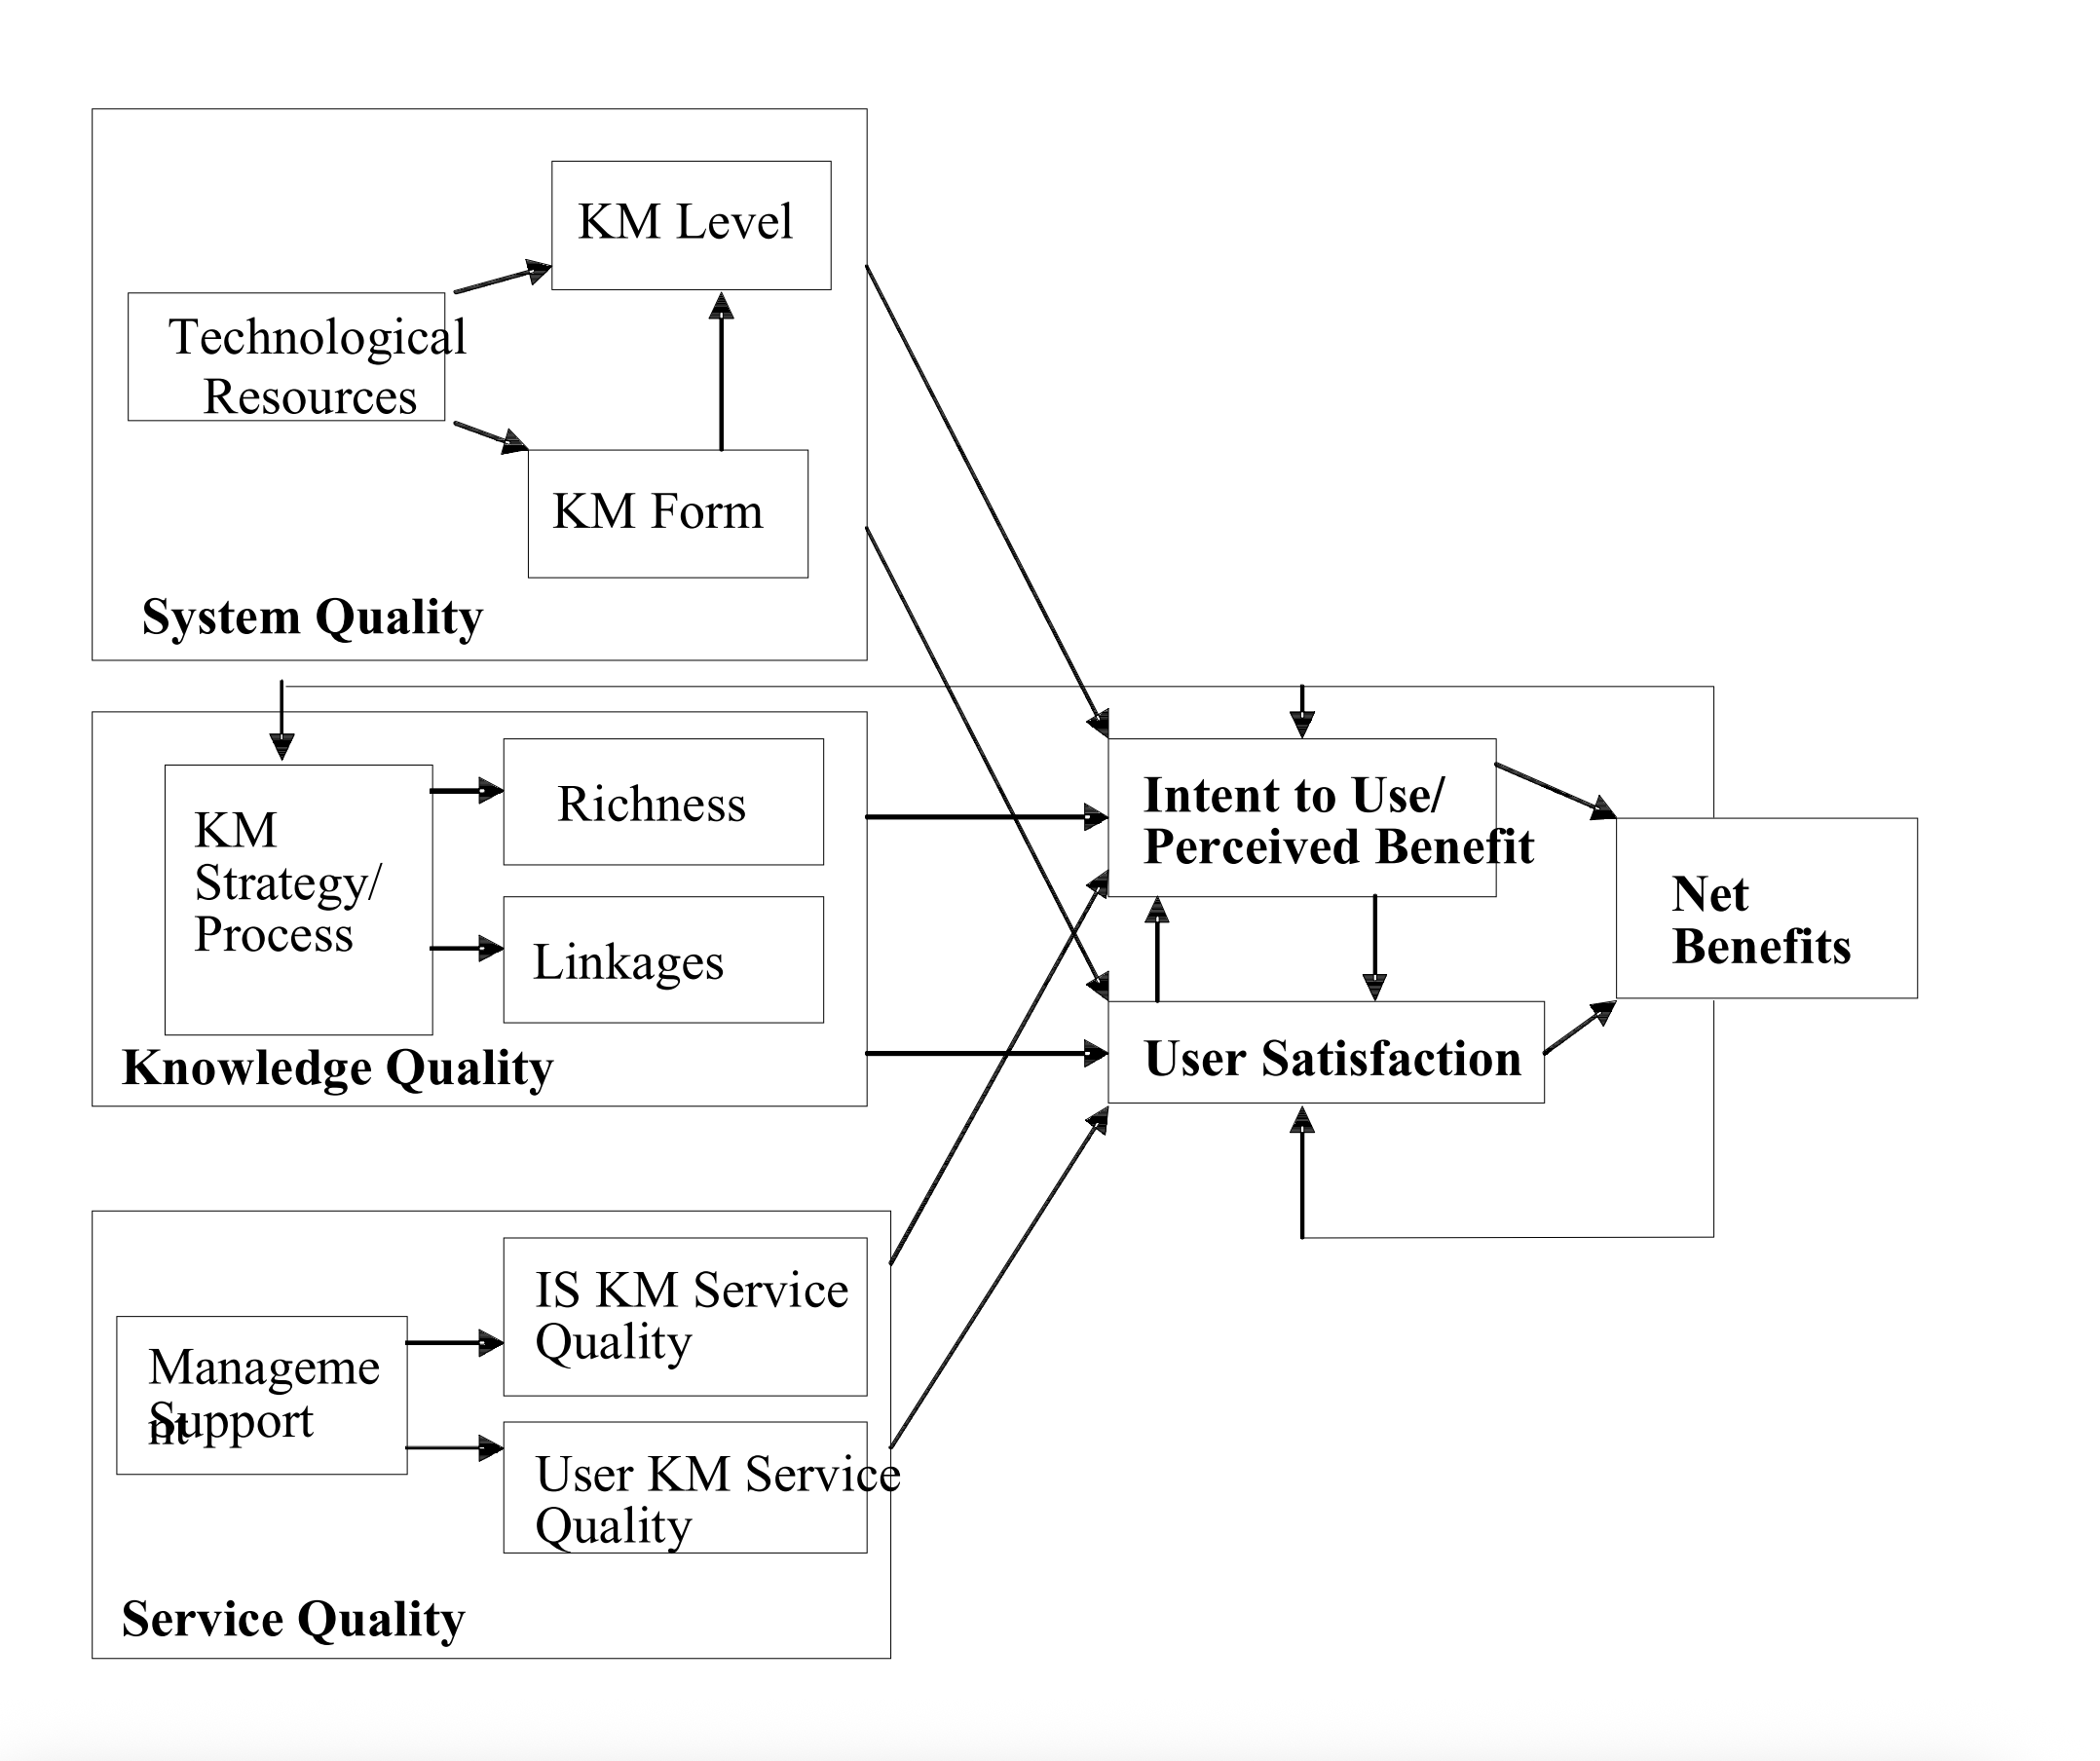
\includegraphics[width=1\linewidth]{knowledge_management_success.png}
    \caption{Knowledge management success model by Jennex & Olfman}
    \label{fig:enter-label}
\end{figure}
The \textit{System Quality} dimension now extends to contain the \textit{technological resources}, \textit{KM form} and the \textit{KM level}. \textit{Technological resources} define the capability of an organization to develop, operate, and maintain KM. This includes all kinds of technical conditions like the amount of experience available to develop, operate and maintain the KM, the underlying network infrastructure or the databases to hold the data use in KM. The \textit{KM form} refers to the extent to which knowledge and knowledge management processes are computerized and integrated. This is important since computerized KM processes are more effective than analogue ones as they make knowledge accessible everywhere at any time through a simple to use interface. The \textit{KM level} in the end refers to the ability to influence current activities. \textit{Technological resources} and the \textit{KM form} are both enablers for the \textit{KM level} and serve as a technical foundation for the ability of the KMS to influence the decision-making process.\\\\
The \textit{Knowledge Quality· dimension} consists of three subsidiary factors too - the \textit{KM strategy/process}, the \textit{Richness} of the captured knowledge and the \textit{Linkages} among the knowledge components. The \textit{Knowledge strategy/process} factor is the basis for the two other factors and means looks at the organizational processes organizing the knowledge management and to which extend these processes are formalized. \textit{Richness} on the other hand evaluates the accuracy and timeliness of the knowledge itself - one could say it is the quality of the actual knowledge. Linkages refer to how accessible the knowledge is through things like knowledge and topic maps etc.\\\\
The \textit{service quality} dimension determines if users of the KMS are provided with sufficient support to use the KMS effectively. It consists of three parts aswell. The \textit{management support} refers to the provision of adequate resources for the KM the organization aswell as the creation of knowledge-sharing organization culture by the organization's management. User KM service quality refers to the support provided by the user organization in order to train the users to use the KMS effectively. On the other hand the IS KM service quality refers to the support provided by the  IS organization to allow users to use the KM aswell as maintaining it. This includes the building, setup and maintaining the KM infrastructure ensuring availability, reliability and security of the KMS provided.\\\\
All three dimensions - the \textit{system quality}, \textit{knowledge quality} and the \textit{service quality} influence similar to the original ISSS the \textit{Intention to use and usage} aswell as the \textit{User Satisfaction} and cause a \textit{net benefit} in the end.
\section{RAG Systems in enterprises}
Since we now know what determines the success of KMS in organizations like enterprises, we are going to have a closer look at the GenAI systems that are used to support KM in an organization, find out what they are used for and which factors define their quality.\\
The GenAI system that we are going to focus on throughout this thesis is a retrieval augmented generation (RAG) system. These systems utilize external data sources like web pages, other organizational KMS or third-party sources through retrieval algorithms, and pass the retrieved knowledge to large language models (LLM) that generate answers grounded on the retrieved knowledge. As such RAG systems can be used for knowledge retrieval and provide advantages for this task.\\
One problem of LLMs that do not use RAG is that they can only provide the data that they were trained on. This causes them to become out-dated. As we know from the KMS success model it is crucial for an organization to be able to access up-to-date information using their KMS. RAG systems can provide this by utilizing up-to-date knowledge sources for their generation.\\
Another issue of LLMs is that they tend to hallucinate if they don't know the answer to a users query or apply a pattern from the training data in a wrong way. Since RAG systems bound the LLMs they use to the information provided by the retrieval algorithms, they reduce hallucinations and a user is always able to verify the answer provided by the LLM by double-checking the sources that were used by the RAG system. This way the RAG approach improves the accuracy of LLMs.\\
Since RAG systems are able to query various data sources at once, they provide good linkages to other KMS as well. Following the KM success model RAG systems seem like a pretty good choice when it comes to KM.\\
However, RAG systems need some effort to serve these qualities to their users in the organizations practice. One of the major challenges is the underlying data that is used for the RAG system. These data are usually not optimized for the use by a RAG system which poses a lot of challenges to the operators of the system. One example for these challenges are vast and complex knowledge bases that on the one hand lead to poor performance - bad \textit{system performance} - since the retrieval algorithms have to perform on a huge dataset and on the other hand pose challenges regarding the integration of them (\textit{service quality}) since various APIs have to be connected to the RAG system. Enterprises usually need a very high accuracy as well because their decision-making processes involve important legal or financial decisions and if a RAG system fails to meet the required accuracy, e.g. because the retrieval algorithms are not able to gather the requested information from the huge and complex dataset, this can lead to a poor \textit{net benefit} of the system. RAG systems like any other GenAI technology are new to most end users too and require training \textit{(service quality)} in order to allow users to use them effectively. In the end we can conclude that RAG systems provide a huge potential at enhancing an organizations KM, but they need a lot of effort to realize it. The goal of this thesis is to support organizations with the realization of RAG applications potential by providing system administrators valuable insights into the usage of the systems.\\
%---------------------------------------------------------------------%
%------------------------------ Methodology --------------------------%
%---------------------------------------------------------------------%
\chapter{Methodology}
The research methodology is based on the DSR approach, which involves both the development and the evaluation of artifacts in iterative cycles. DSR aims to develop innovative solutions for specific problems and to test these solutions in real-world contexts (Peffers et al., 2007b, p. 4).\\
\subsection{Problem Identification and Motivation}
In the first phase of the DSR approach, the need for support in managing the RAG system was identified. It was determined that system administrators require insights that allow them to better assess the current performance and quality of the RAG application and to draw conclusions about which measures must be taken to improve it. Examples of such measures could be employee training, improving the knowledge base, or enhancing the RAG mechanism itself.
\section{First iteration - Definition of valuable insights}
In the first iteration, specific software features were defined to support system administrators in managing the system. This was done in collaboration with the developers of the RAG software under investigation during several joint workshops.
\subsection{Define Objectives of Artifacts}
In a first workshop, initial ideas for evaluating the RAG application were collected, and its current data situation was analyzed to determine what additional data must be gathered to implement the automated analysis. The developers were presented with the foundational principles of Information Systems Success (ISSS) and Knowledge Management Systems (KMS) success. They then developed ideas related to both topics in small groups and afterwards discussed their findings in a plenary session. Through this process, the objectives for the evaluation of the RAG system were clearly established
\subsection{Development of Artifacts}
Based on the developers' ideas, specific concepts for software features were developed and then classified into the quality categories of the IS Success Model (ISSM).
\subsection{Demonstration and Evaluation}
In a second workshop, the developed concepts were presented to the developers and feedback on them was gathered. Additionally, the individual software features were prioritized to ensure that the subsequent implementation phase could focus on developing and delivering the most important ones.
\section{Second iteration - Implementation of insights}
In the second iteration, the developed software features were technically implemented and integrated into the existing RAG application.
\subsection{Define Objectives of Artifacts}
First, various solutions for the technical implementation were developed and presented once again to the development team. Feedback was gathered, and a decision was made on how the features should be technically implemented.
\subsection{Development of Artifacts}
Subsequently, the software features were implemented and integrated into the existing RAG application. This was done using an iterative software development process (Scrum). Technical reviews took place to validate the correctness of the created software features.
\subsection{Demonstration and Evaluation}
Finally, the created software features were presented to the development team in a final workshop and feedback was gathered.
%---------------------------------------------------------------------%
%------------------------------ Results ------------------------------%
%---------------------------------------------------------------------%
\chapter{Results}
In the following chapter we are going to elaborate on the conecpts of the software features created during the workshops and how they have been implemented in the RAG application. The feedback of the developer team will be discussed as well.
\section{Description of the RAG system used in the study}

\section{Software features}
\subsection{Measurements of the system quality}
\subsubsection{Response times}
To determine the system performance, it is crucial to measure the time it takes from the initiation of a request until the answer is generated completely. Yet the response time should always be connected with 
\subsubsection{Error rates}
\subsection{Measurements of the knowledge quality}
\subsubsection{Topic maps}
\subsubsection{Task type maps}
\subsubsection{Quality of the retrieval and the generated responses}
\subsubsection{Combining quality with task types and topics}
\subsubsection{Combination of task type and topics}
\subsection{Measurements of the service quality}
\subsubsection{Interactivity}
\subsubsection{Knowledge gap detection}
\section{Description of the technical implementation of the software features}
\subsubsection{Topic maps}
\subsubsection{Task type maps}
\subsubsection{Quality of the retrieval and the generated responses}
\subsubsection{Combining quality with task types and topics}
\subsubsection{Combination of task type and topics}

\section{Final feedback from the development team}

%---------------------------------------------------------------------%
%------------------------------ Discussion ---------------------------%
%---------------------------------------------------------------------%
\chapter{Discussion}

%---------------------------------------------------------------------%
%---------------------------- Conclusion -----------------------------%
%---------------------------------------------------------------------%
\chapter{Conclusion}
Lorem ipsum dolor sit amet, consetetur sadipscing elitr, sed diam nonumy eirmod tempor invidunt ut labore et dolore magna aliquyam erat, sed diam voluptua. At vero eos et accusam et justo duo dolores et ea rebum. Stet clita kasd gubergren, no sea takimata sanctus est Lorem ipsum dolor sit amet. Lorem ipsum dolor sit amet, consetetur sadipscing elitr, sed diam nonumy eirmod tempor invidunt ut labore et dolore magna aliquyam erat, sed diam voluptua. At vero eos et accusam et justo duo dolores et ea rebum. Stet clita kasd gubergren, no sea takimata sanctus est Lorem ipsum dolor sit amet. Lorem ipsum dolor sit amet, consetetur sadipscing elitr, sed diam nonumy eirmod tempor invidunt ut labore et dolore magna aliquyam erat, sed diam voluptua. At vero eos et accusam et justo duo dolores et ea rebum. Stet clita kasd gubergren, no sea takimata sanctus est Lorem ipsum dolor sit amet.
\section{Blindtext Überschrift Ebene 2 Blindheit per Definition}
Mit Blindheit per Definition geschlagen, dennoch nicht unsichtbar, präsentiere ich mich als unbeachtetes und ungeliebtes Stiefkind zeitgenössischer Literatur. Meine Bestimmung liegt - wie ich selbst - in engen Grenzen und ist rein platzhalterischer Natur. Kann ein missbrauchtes Wortgefüge eigentlich noch Schlimmeres erleiden, als als Blindtext erdacht und vor der Öffentlichkeit versteckt zu werden?
\subsection{Blindtext Überschrift Ebene 3}
Ut wisi enim ad minim veniam, quis nostrud exerci tation ullamcorper suscipit lobortis nisl ut aliquip ex ea commodo consequat. Duis autem vel eum iriure dolor in hendrerit in vulputate velit esse molestie consequat, vel illum dolore eu feugiat nulla facilisis at vero eros et accumsan et iusto odio dignissim qui blandit praesent luptatum zzril delenit augue duis dolore te feugait nulla facilisi.\\
Nam liber tempor cum soluta nobis eleifend option congue nihil imperdiet doming id quod mazim placerat facer possim assum. Lorem ipsum dolor sit amet, consectetuer adipiscing elit, sed diam nonummy nibh euismod tincidunt ut laoreet dolore magna aliquam erat volutpat. Ut wisi enim ad minim veniam, quis nostrud exerci tation ullamcorper suscipit lobortis nisl ut aliquip ex ea commodo consequat.\\
Duis autem vel eum iriure dolor in hendrerit in vulputate velit esse molestie consequat, vel illum dolore eu feugiat nulla facilisis.
\subsection{Blindtext Überschrift Ebene 3 Inhaltsleer}
Streng dem definierten Wesen des Blindtextes folgend, fungiere ich als solcher und gebe mich unverbindlich inhaltsleer. In bedrückender Enge in vorgefertigte Masken gepresst friste ich ein freudloses Dasein auf dem schmalen Grat zwischen Nichtbeachtung und Bedeutungslosigkeit und habe doch eine Bitte: Handeln Sie Sinn stiftend für meine Existenz und lesen Sie mich.
\section{Blindtext Überschrift Ebene 2}
Lorem ipsum dolor sit amet, consetetur sadipscing elitr, sed diam nonumy eirmod tempor invidunt ut labore et dolore magna aliquyam erat, sed diam voluptua. At vero eos et accusam et justo duo dolores et ea rebum. Stet clita kasd gubergren, no sea takimata sanctus est Lorem ipsum dolor sit amet. Lorem ipsum dolor sit amet, consetetur sadipscing elitr, sed diam nonumy eirmod tempor invidunt ut labore et dolore magna aliquyam erat, sed diam voluptua. At vero eos et accusam et justo duo dolores et ea rebum. Stet clita kasd gubergren, no sea takimata sanctus est Lorem ipsum dolor sit amet. Lorem ipsum dolor sit amet, consetetur sadipscing elitr, sed diam nonumy eirmod tempor invidunt ut labore et dolore magna aliquyam erat, sed diam voluptua. At vero eos et accusam et justo duo dolores et ea rebum. Stet clita kasd gubergren, no sea takimata sanctus est Lorem ipsum dolor sit amet.\\
Duis autem vel eum iriure dolor in hendrerit in vulputate velit esse molestie consequat, vel illum dolore eu feugiat nulla facilisis at vero eros et accumsan et iusto odio dignissim qui blandit praesent luptatum zzril delenit augue duis dolore te feugait nulla facilisi. Lorem ipsum dolor sit amet, consectetuer adipiscing elit, sed diam nonummy nibh euismod tincidunt ut laoreet dolore magna aliquam erat volutpat \parencite{emse-03339298, koppe2021herausforderungen}.\\
Ut wisi enim ad minim veniam, quis nostrud exerci tation ullamcorper suscipit lobortis nisl ut aliquip ex ea commodo consequat. Duis autem vel eum iriure dolor in hendrerit in vulputate velit esse molestie consequat, vel illum dolore eu feugiat nulla facilisis at vero eros et accumsan et iusto odio dignissim qui blandit praesent luptatum zzril delenit augue duis dolore te feugait nulla facilisi.\\
\section{Blindtext Überschrift Ebene 2 Gummibärchen}
Freilebende Gummibärchen gibt es nicht. Man kauft sie in Packungen an der Kinokasse. Dieser Kauf ist der Beginn einer fast erotischen und sehr ambivalenten Beziehung Gummibärchen-Mensch. Zuerst genießt man. Dieser Genuss umfasst alle Sinne. Man wühlt in den Gummibärchen, man fühlt sie. Gummibärchen haben eine Konsistenz wie weichgekochter Radiergummi. Die Tastempfindung geht auch ins Sexuelle. Das bedeutet nicht unbedingt, dass das Verhältnis zum Gummibärchen ein geschlechtliches wäre, denn prinzipiell sind diese geschlechtsneutral. Nun sind Gummibärchen weder wabbelig noch zäh; sie stehen genau an der Grenze. Auch das macht sie spannend. Gummibärchen sind auf eine aufreizende Art weich. Und da sie weich sind, kann man sie auch ziehen. Ich mache das sehr gerne. Ich sitze im dunklen Kino und ziehe meine Gummibärchen in die Länge, ganz ganz langsam. Man will sie nicht kaputtmachen, und dann siegt doch die Neugier, wie viel Zug so ein Bärchen aushält. (Vorstellbar sind u. a. Gummibärchen-Expander für Kinder und Genesende). Forscherdrang und gleichzeitig das Böse im Menschen erreichen den Climax, wenn sich die Mitte des gezerrten Bärchens von Millionen Mikrorissen weiß färbt und gleich darauf das zweigeteilte Stück auf die Finger zurückschnappt. Man hat ein Gefühl der Macht über das hilflose, nette Gummibärchen. Und wie man damit umgeht: Mensch erkenne dich selbst! Jetzt ist es so, dass Gummibärchen ja nicht gleich Gummibärchen ist. Ich bevorzuge das klassische Gummibärchen, künstlich gefärbt und aromatisiert. Mag sein, dass es eine Sentimentalität ist. Jedenfalls halte ich nichts von neuartigen Alternativ-Gummibärchen ohne Farbstoff (»Mütter, mit viel Vitamin C«), und auch unter den konventionellen tummeln sich schwarze Schafe: die schwarzen Lakritz-Bärchen. Wenn ich mit Xao im Kino bin, red ich ihm so lange ein, dass das die besten sind, bis er sie alle isst. Sie schmecken scheußlich und fühlen sich scheußlich an. Dagegen das schöne, herkömmliche Gummibärchen: allein wie es neonhaft vom Leinwandleuchten illuminiert, aber ganz ohne die Kühle der Reklameröhren! Die nächste prickelnde Unternehmung ist das Kauen des Gummibärchens \parencite{arbelaez2010contour}. Es ist ein Katz-und-Maus-Spiel. Man könnte zubeißen, lässt aber die Spannung noch steigen. Man quetscht das nasse Gummibärchen zwischen Zunge und Gaumen und glibscht es durch den Mund. Nach einer Zeit beiße ich zu, oft bei nervigen Filmszenen. Es ist eine animalische Lust dabei. Was das schmecken angeht. wirken Gummibärchen in ihrer massiven Fruchtigkeit sehr dominierend. Zigaretten auf Gummibärchen schmecken nicht gut. Anführen sollte man auch noch: manche mögen die Grünen am liebsten, manche die Gelben. Ich mag am liebsten die Roten. Sie glühen richtig rot, und ihr Himbeergeschmack fährt wie Napalm über die Geschmacksknospen. Eine meiner Lieblingsphantasien, wo es um Gummibärchen geht, ist der Gummibär. Ich will einen riesigen Gummibären. Jeder wahre Gummibärchen-Gourmet wird mich verstehen. Ebenfall fantasieanregend können sie eingesetzt werden zum Aufbau verschiedener »Orgiengruppen- Modelle« oder als »Demonstrationsobjekt für wirbellose Tiere«. Abgesehen vom diabolischen Lustgewinn müsste man die Bärchen gar nicht zerreißen. Sie sind ja durchscheinend. Zu behaupten, dass sich im Gummibärchen das Wesen aller Dinge offenbart, finde ich keinesfalls als gewagt. Wer schon einmal über einem roten Gummibärchen meditiert hat, weiß von diesen Einsichten. Wenn ich das Kino verlasse oder die Packung einfach leergegessen ist, habe ich meist ein Gefühl, als hätte mir einer in den Magen getreten. Hier schläft die gesteigerte Intensität - als deren Ursache den Gummibärchen durchaus der Charakter einer Droge zuerkannt werden kann - ins Negative um, in den Überdruss. In dichter und geraffter Form spiegelt sich im Verhältnis zum Gummibärchen eine menschliche Love-Affair wider. Nie wieder Gummibärchen, denke ich jedes Mal. In der Zwischenzeit lächle ich dann über den Absolutheitsanspruch den diese Momente erheben. Schon zu Hause beunruhigen mich wieder Gerüchte über einen Marktvorstoß der Japaner mit Gummireis oder Gummischweinen. Und wieder und wieder geht es mir durch den Kopf: Gummibärchen sind Spitze.

%---------------------------------------------------------------------%
%------------------------------ Appendix -----------------------------%
%---------------------------------------------------------------------%
\chapter*{Anhang}
\addcontentsline{toc}{chapter}{Anhang}           %Kapitel bekommt keine Nummerierung und wird trotzdem
                                                                %ins Inhaltsverzeichnis aufgenommen
% Fortsetzung der römischen Seitennummerierung
\pagenumbering{Roman}
\setcounter{page}{\value{seitenzahlroemisch}}




\printbibliography



%\affidavit


\end{document}
